%%%%%%%%%%%%%%%%%%%%%%% file typeinst.tex %%%%%%%%%%%%%%%%%%%%%%%%%
%
% This is the LaTeX source for the instructions to authors using
% the LaTeX document class 'llncs.cls' for contributions to
% the Lecture Notes in Computer Sciences series.
% http://www.springer.com/lncs       Springer Heidelberg 2006/05/04
%
% It may be used as a template for your own input - copy it
% to a new file with a new name and use it as the basis
% for your article.
%
% NB: the document class 'llncs' has its own and detailed documentation, see
% ftp://ftp.springer.de/data/pubftp/pub/tex/latex/llncs/latex2e/llncsdoc.pdf
%
%%%%%%%%%%%%%%%%%%%%%%%%%%%%%%%%%%%%%%%%%%%%%%%%%%%%%%%%%%%%%%%%%%%


% \documentclass[runningheads,a4paper]{llncs}
\documentclass[a4paper]{llncs}

\usepackage{multirow,enumerate,array,float}
\usepackage{amssymb}
\setcounter{tocdepth}{3}
\usepackage{graphicx}
\graphicspath{ {./figures/} }

\usepackage{url}
\urldef{\mailsa}\path|keyanp@cs.washington.edu|
\newcommand{\keywords}[1]{\par\addvspace\baselineskip
\noindent\keywordname\enspace\ignorespaces#1}

\begin{document}

\mainmatter  % start of an individual contribution

% first the title is needed
\title{Improving healthcare outcomes and cost through analysis and design of provider incentives}

% a short form should be given in case it is too long for the running head
% \titlerunning{Improving healthcare outcomes}

% the name(s) of the author(s) follow(s) next
%
% NB: Chinese authors should write their first names(s) in front of
% their surnames. This ensures that the names appear correctly in
% the running heads and the author index.
%
\author{Keyan Pishdadian}
%
% \authorrunning{Improving healthcare outcomes}
% (feature abused for this document to repeat the title also on left hand pages)

% the affiliations are given next; don't give your e-mail address
% unless you accept that it will be published
\institute{University of Washington\\
\mailsa
}

%
% NB: a more complex sample for affiliations and the mapping to the
% corresponding authors can be found in the file "llncs.dem"
% (search for the string "\mainmatter" where a contribution starts).
% "llncs.dem" accompanies the document class "llncs.cls".
%

% \toctitle{Lecture Notes in Computer Science}
% \tocauthor{Authors' Instructions}
\maketitle


\begin{abstract}
Provider decision making plays a critical role in patient outcomes and national healthcare spending. Creating robust incentive structures to underlie provider deicision making are vital to ensuring the delivery of high quality care and adequately managed costs. Despite this these incentive structures are poorly designed both financially and from a provider risk perspective. In this paper we analyze the inefficiencies and sub-optimal equilibria that result from the use of classic incentive systems, then extend recent ideas to propose a hybrid incentive structure that increases provider profits, improves patient outcomes, and reduces wasteful spending.

\keywords{health care economics, incentives, game theory, prisioner's dilemma, US health care system}
\end{abstract}


\section*{Introduction}

Healthcare is a socially and economically important aspect of the modern United States. Roughly 1/6th of US consumer spending \cite{econharvard} and ~48\% of federal spending \cite{federalspend} goes towards some form of healthcare and the success, efficiency, and outcomes of this market reflect directly on the viability and happiness of American citizens and the US economy. The decision making of physicians plays a integral role in this system, with roughly 80\% of all expenditure being a result of physicians' decisions \cite{trust}. One becomes concerned with this control when comparing US healthcare expenditure to other developed countries (Fig. \ref{fig:usspend}), just why is expenditure so much higher then? At the root of the issue is that the healthcare market is unlike other normal markets where there is a buyer and a seller, with the buyer fully knowing what it is they want and having transparency into the price being offered by the seller \cite{msdt}. Rather in this market there are many agents interacting directly or indirectly within a single healthcare transaction. We summarize these agents below (note that to simplify the model we ignore altruistic behavior and moral incentives):

\begin{itemize}
    \item \textbf{patient}: who seeks to minimize cost to themselves, while maximizing quality of service
    \item \textbf{provider}: who seeks to maximize revenue to themselves, while minimizing volume of services rendered, and also minimizing financial and professional risk (e.g. malpratice lawsuits, increased cost of caring of patient with worsened condition)
    \item \textbf{hospital}: who seeks to maximize revenue, while minimizing cost and volume of service
    \item \textbf{other providers}: who act the same as the main provider, but whose actions have positive or negative externalities on the global wellbeing of the patient population.
\end{itemize}

Unfortunately the classic incentive structures used result in a complex web of interdependencies between the agents (Fig. \ref{fig:agentdep}).

At the root of the issue is the fact that the patient-provider relationship is a clear example of a \emph{principle-agent problem} \cite{principle} where the provider (the ``agent") must make diagnosis and care decisions that impact the patient (the ``principle"), but 

a principle-agent problem between providers (agents) and payers (government/insurance companies), as well as multiple ``prisoners' dilemmas" between providers and patients as well as providers and other providers \cite{blended}. In this paper we analyze the inefficiencies and sub-optimal equilibria that result from the use of classic incentive systems, then extend recent ideas to propose a hybrid incentive structure that increases provider profits and improves patient outcomes.\footnote{The footnote numeral is set flush left and the text follows with the usual word spacing.}


\begin{table}[H]
\centering
  \setlength{\extrarowheight}{2pt}
  \begin{tabular}{*{4}{c|}}
    \multicolumn{2}{c}{} & \multicolumn{2}{c}{Player II (even)}\\\cline{3-4}
    \multicolumn{1}{c}{} &  & $2$  & $3$ \\\cline{2-4}
    \multirow{2}*{Player 1 (odd)}  & $2$ & $(-4,4)$ & $(6,-6)$ \\\cline{2-4}
    & $3$ & $(6,-6)$ & $(-9,9)$ \\\cline{2-4}
  \end{tabular}
\caption{Payoff matrix zero-sum number calling game.}
\end{table}

\begin{figure}
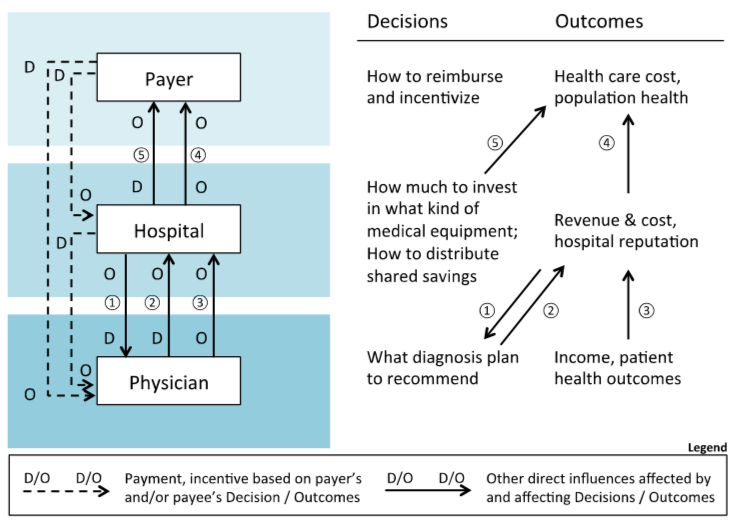
\includegraphics[height=7cm]{agentdep}
\centering
\caption{Agent interdepence diagram which shows the complex network of interactions between patients (Payer), providers (Physician), and hospitals. In this work we focus on controlling the decision making process (relations $1$ and $2$) and patient health outcomes and cost (relation $4$) \cite{msdt}.}
\label{fig:agentdep}
\end{figure}

\begin{figure}
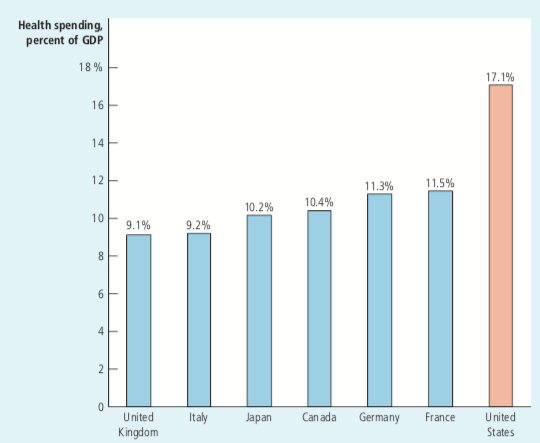
\includegraphics[height=7cm]{usspend}
\centering
\caption{US healthcare expenditure is significantly higher than that of other developed countries}
\label{fig:usspend}
\end{figure}

\begin{figure}
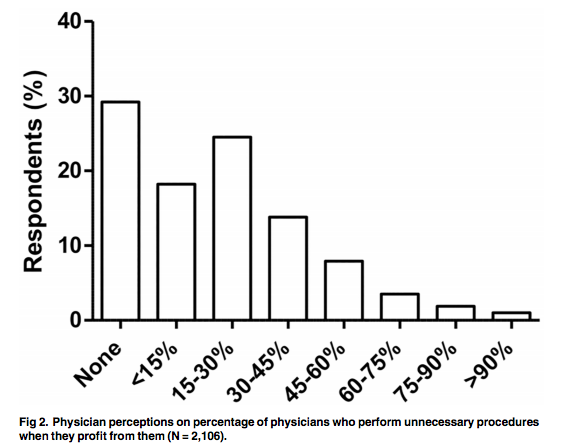
\includegraphics[height=7cm]{overtreat}
\centering
\caption{Provider responses when surveyed and asked what percentage of other physicians they think perform uneeded procedures financial gain \cite{overtreat}}
\label{fig:overtreat}
\end{figure}


\section*{Background}

\subsection*{Fee-for-service}
Foo bar baz

\subsection*{Capitation}
Foo bar baz

\subsection*{Accountable Care Organizations}
Foo bar baz

\section*{Modeling Incentives}

\section*{Hybrid Approach}


%--------------------------------- Bibliography ----------------------------------

\begin{thebibliography}{8}

\bibitem{federalspend}
The True Cost of Health Care: An Analysis of Americans’ Total Health Care Spend
\\\texttt{https://bit.ly/39wbFzi}

\bibitem{econharvard}
Mankiw NG. (2017) The Economics of Healthcare.

%6
\bibitem{trust}
Djulbegovic, Benjamin \& Hozo, Iztok \& Ioannidis, John. (2014). Modern health care as a game theory problem. European Journal of Clinical Investigation. 45. 10.1111/eci.12380

\bibitem{tim}
Roughgarden, T. (2016). Asymmetric Information and Reputation Systems. \texttt{http://timroughgarden.org/f16/l/l12.pdf}

\bibitem{overtreat}
Lyu H, Xu T, Brotman D, Mayer-Blackwell B, Cooper M, Daniel M, et al. (2017). Overtreatment in the United States. PLoS ONE 12(9): e0181970. https://doi.org/10.1371/journal.pone.0181970

% 1
\bibitem{inflation}
Agee, M.D., Gates, Z. (2013). Lessons from Game Theory about Healthcare System Price Inflation. Appl Health Econ Health Policy 11, 45–51. https://doi.org/10.1007/s40258-012-0003-z

%7
\bibitem{tarrant}
Tarrant, C., Stokes, T., \& Colman, A. M. (2004). Models of the medical consultation: opportunities and limitations of a game theory perspective. Quality \& safety in health care, 13(6), 461–466. doi:10.1136/qhc.13.6.461kj

%4
\bibitem{blended}
DeVoe, J. E., \& Stenger, R. (2013). Aligning provider incentives to improve primary healthcare delivery in the United States. OA family medicine, 1(1), 7. doi:10.13172/2052-8922-1-1-958

%5
\bibitem{msdt}
Zhang, H., Wernz, C. \& Slonim, A.D. (2016). Aligning incentives in health care: a multiscale decision theory approach. EURO J Decis Process 4, 219–244. https://doi.org/10.1007/s40070-015-0051-3

%2
\bibitem{mindyour}
Prisoners dilemma and doctor prescribing, \texttt{https://bit.ly/330YC6z}

\bibitem{principle}
Eisenhardt, K. (1989). Agency Theory: An Assessment and Review. The Academy of Management Review, 14(1), 57-74. www.jstor.org/stable/258191

\end{thebibliography}

%-------------------------------------------------------------------

\end{document}
